% Circumscribed Parallelepiped
% Author: Axel Pavillet
\documentclass[border=10pt]{standalone}
\usepackage{tkz-graph}
\usepackage{relsize}
\usetikzlibrary{arrows,decorations.markings,calc}

\definecolor{cd40000}{RGB}{212,0,0}
\definecolor{cffffff}{RGB}{255,255,255}
\definecolor{c2a7fff}{RGB}{42,127,255}
\definecolor{c0000d9}{RGB}{0,0,217}
\definecolor{c0000ff}{RGB}{0,0,255}

\usepackage{relsize}

\tikzset{every path/.style={draw,>=latex,line width=1pt,color=black}}

%\tikzset{every node/.style={draw,minimum width = 20pt,line width = 1.75pt,
%circle,inner sep=0pt,font = \fontsize{14}{14}\selectfont,fill=none}}

\begin{document}
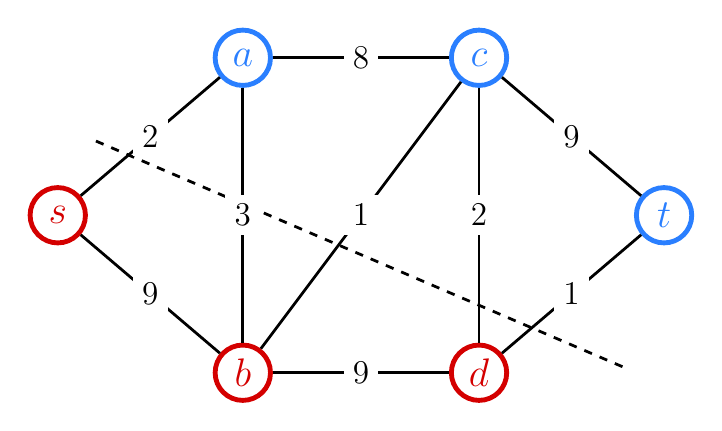
\begin{tikzpicture}[scale=0.5]
\begin{scope}[every node/.style={draw,minimum width = 20pt,line width = 1.75pt,
circle,inner sep=0pt,font = \fontsize{14}{14}\selectfont,fill=none}]
\node[color=cd40000] (s) at (-0.7,4) {$s$};
\node[color=c2a7fff] (t) at (14.7,4) {$t$};
%\node (e) at (7,4) {$e$};
\node[color=c2a7fff] (a) at (4,8) {$a$};
\node[color=c2a7fff] (c) at (10,8) {$c$};
\node[color=cd40000] (b) at (4,0) {$b$};
\node[color=cd40000] (d) at (10,0) {$d$};
\end{scope}

\begin{scope}
\node[color=white] (a1) at (0,6) {};
\node[color=white] (a2) at (14,0) {};
\end{scope}

\begin{scope}
\tikzset{every path/.style={draw,dashed,>=latex,line width=1pt,color=black}}
\path (a1) -- (a2);
\end{scope}

\path[-] (s) -- (a) node[midway, fill=white, font=\fontsize{12}{12}\selectfont] {$2$};
\path[-] (s) -- (b) node[midway, fill=white, font=\fontsize{12}{12}\selectfont] {$9$};
%\path[->] (s) -- (e) node[midway, fill=white, font=\fontsize{12}{12}\selectfont] {$12$};
\path[-] (b) -- (a) node[midway, fill=white, font=\fontsize{12}{12}\selectfont] {$3$};
\path[-] (c) -- (a) node[midway, fill=white, font=\fontsize{12}{12}\selectfont] {$8$};
\path[-] (c) -- (b) node[midway, fill=white, font=\fontsize{12}{12}\selectfont] {$1$};
% \draw[->] (a) to [bend left=20]  node[midway, fill=white, font=\fontsize{12}{12}\selectfont] {$6$} (c);
% \draw[->] (c) to [bend left=20]  node[midway, fill=white, font=\fontsize{12}{12}\selectfont] {$6$} (a);
%\path[->] (b) -- (e) node[midway, fill=white, font=\fontsize{12}{12}\selectfont] {$2$};
%\path[->] (e) -- (d) node[midway, fill=white, font=\fontsize{12}{12}\selectfont] {$2$};
\path[-] (b) -- (d) node[midway, fill=white, font=\fontsize{12}{12}\selectfont] {$9$};
\path[-] (d) -- (t) node[midway, fill=white, font=\fontsize{12}{12}\selectfont] {$1$};
\path[-] (c) -- (d) node[midway, fill=white, font=\fontsize{12}{12}\selectfont] {$2$};
\path[-] (c) -- (t) node[midway, fill=white, font=\fontsize{12}{12}\selectfont] {$9$};
%\path[->] (e) -- (t) node[midway, fill=white, font=\fontsize{12}{12}\selectfont] {$1$};

\end{tikzpicture}
\end{document}
